\documentclass[12pt]{article}
\usepackage[margin=1in]{geometry}
\usepackage{amsmath, amssymb, amsthm, graphicx, hyperref}
\usepackage{graphicx}
\usepackage{enumerate}
\usepackage{multirow, multicol}
\usepackage{tikz}
\usepackage{fancyhdr}
\usepackage{algpseudocode}
\pagestyle{fancy}
\usepackage{comment}
\usepackage{float}
\newif\ifshow
\showfalse
\setlength{\parindent}{20pt}

\fancyhead[LO]{Project 1}
\fancyhead[RO]{Wang \& DiPietrantonio} 

\begin{document}

\title{Cryptanalysis of a class of ciphers based on character frequency, grouping, and Levenshtein distance}
\author{Guandi Wang \& Daniel DiPietrantonio}
\maketitle

\pagebreak
%---------------------------------------------------------

\section{Introduction}
This project was completed by Guandi Wang and Daniel DiPietrantonio. Guandi worked heavily on our submission for test 1, and Daniel made minor edits and test scripts to optimize his work. Both team members worked on solutions for test 2, however Guandi's approach proved to be more successful and thus that is what we submitted. Strategies were formulated and devised by both team members. The report was written by both team members.

We are submitting five files for this assignment: the report file, test1 implementation source, test1 implementation binary, test 2 implementation source, and test2 implementation binary. As indicated by the labels, we took a different approach for solving test 1 and test 2. The approach for test 1 was successful, showing a minimal error rate even as the probability of randomness rises. Some errors can be found once the probability approaches 0.5, however it is not unlikely to have successful results even with a probability set to 0.75. The approach for test 2 was successful as well, but less so than test 1. The approach manages to find most of the words with 0 probability of randomness, but struggles as the probability of randomness is raised.

\section{Informal description of approach}
Since we took separate approaches for test 1 and test 2, this section is divided into two subsections. The first talks about our approach, and the second talks about our approach for test 2. Throughout both susections, we talk heavily about character distributions. Included here are plots that show the character distributions of the five plaintexts in dictionary 1 as well as the entire vocabulary in dictionary 2.

\begin{figure}[H]
    \centering
    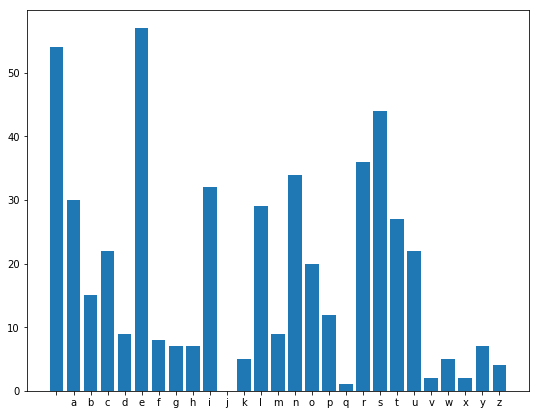
\includegraphics[scale=0.5]{pt1.png}
    \caption{Dictionary 1 - Plaintext 1 Character Frequency}
    \label{fig:pt1}

    \centering
    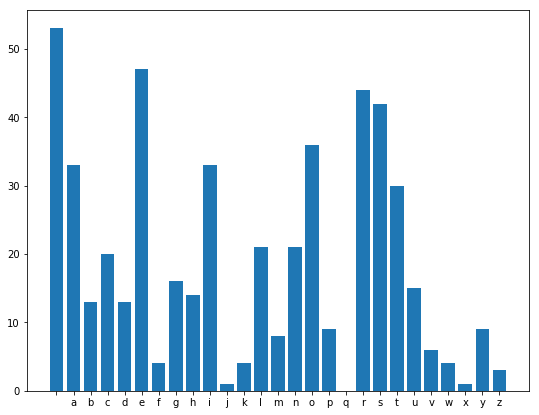
\includegraphics[scale=0.5]{pt2.png}
    \caption{Dictionary 1 - Plaintext 2 Character Frequency}
    \label{fig:pt2}

    \centering
    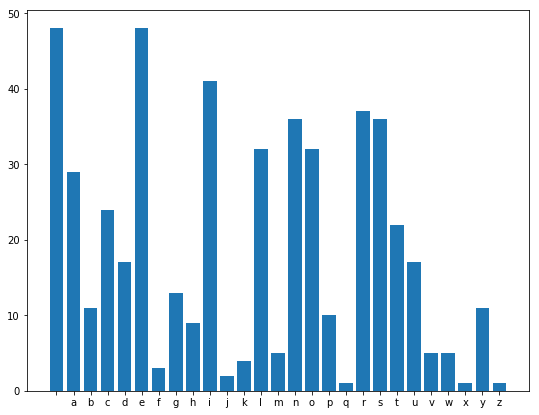
\includegraphics[scale=0.5]{pt3.png}
    \caption{Dictionary 1 - Plaintext 3 Character Frequency}
    \label{fig:pt3}
\end{figure}

\begin{figure}[H]
    \centering
    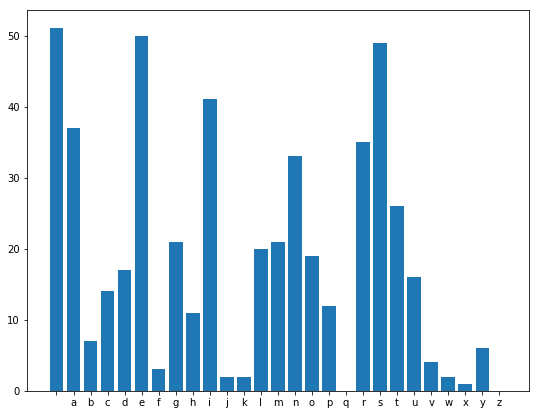
\includegraphics[scale=0.5]{pt4.png}
    \caption{Dictionary 1 - Plaintext 4 Character Frequency}
    \label{fig:pt4}

    \centering
    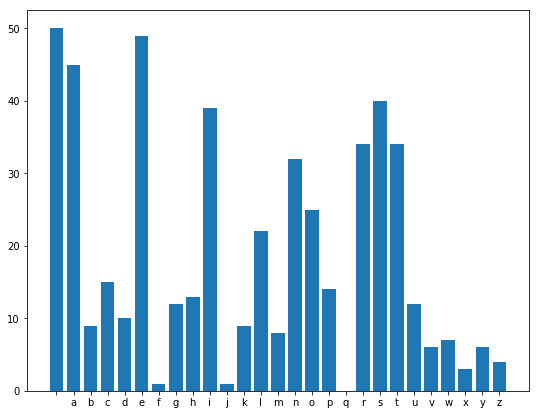
\includegraphics[scale=0.5]{pt5.png}
    \caption{Dictionary 1 - Plaintext 5 Character Frequency}
    \label{fig:pt5}

    \centering
    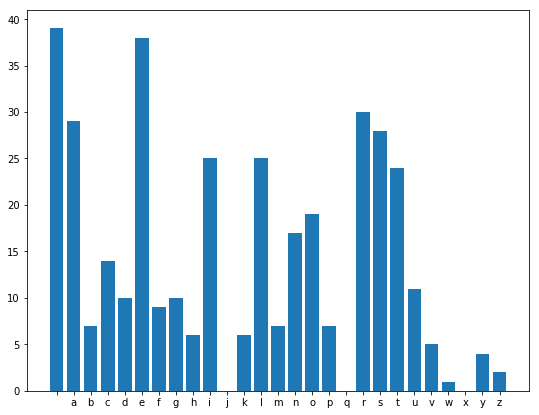
\includegraphics[scale=0.5]{dict2.png}
    \caption{Dictionary 2 Character Frequency}
    \label{fig:dict2}
\end{figure}


\subsection{Approach 1 - Test 1}
At a high level, our approach to test 1 was the following:
\begin{enumerate}

    \item Get the character frequency distribution of the encrypted input text.
    \item Map characters with similar frequencies to the same symbol (grouping stage).
    \item For each character in the input, change that character to the symbol it maps to. We refer to this new symbol-substituted input as the \emph{symbolized input}.
    \item Repeat the above three steps for each candidate plaintext in dictionary 1, creating five symbolized candidate plaintexts.
    \item For each symbolized candidate plaintext, compute the Levenshtein distance (\href{https://en.wikipedia.org/wiki/Levenshtein_distance}{wiki}) between it and the symbolized input.
    \item Output the answer as the candidate plaintext with the minimum Levenshtein distance as computed in step 5.

\end{enumerate}

With a high level understanding of the approach, we can now go into more detail on our implementation. Our approach for test 1 was based on the character frequency distribution of the potential input strings. First, we performed a character frequency analysis of each character in the encrypted input string. This is done by iterating through the input one character at a time, and keeping track of how many times we encountered that counter via a hash map.

After this, we perform a "grouping" step. The inspiration behind this step is the following observation: as more and more random characters are inserted into the encrypted text, the encrypted text's character distribution will become more and more uniform. Therefore, it is not enough to simply match the most commonly occuring character in the encrypted input to the most commonly occuring character in each of the five plaintexts. To fix this, the grouping step matches characters that have similar frequencies to the same symbol. For example, Figure~\ref{fig:pt1} shows that 'g' and 'h' occur with very simliar frequency in plaintext 1 of dictionary 1. In the grouping step, they would be mapped to the same symbol, $\alpha$. A hashmap data structure holds the mapping between a character in the input text and its symbol. For our implementation, we found that a group size of two works best. To make the groups, we sort the characters by frequency, and group them in pairs of two, from least frequent to most frequent. Since there are an odd number of characters in our input alphabet (26 letters and space), the most frequently observed character is mapped to its own symbol.

Once we have our input symbol mapping, we create the \emph{symbolized input}, which is simply a string $S$ of length $L$ (where $L$ is the length of the input) where the $i$th character of $S$ is equal to the symbolized mapping of the $i$th character of the input.

Upon computing our symbolized input string, we now repeat the character frequency analysis, grouping, and symbolized mapping stages (steps $1-3$ in the high level overview) for each of the five candidate plaintexts in dictionary 1, thus giving us one symbolized input and five symbolized candidate plaintexts. 

For each symbolized candidate plaintext, we compute the Levenshtein distance between that symbolized candidate plaintext and the symbolized input string. There were many string comparison algorithms to choose from in this step, however we chose the Levenshtein distance because it outputs the minimum number of character changes between the two strings which is a great metric to compare encrypted text to plaintext. Once we have these five Levenshtein distances, we simply take the minimum of them and output the candidate plaintext whose symbolized plaintext generated that minimum value.

This process is unique in that it doesn't attempt to morph the encrypted text into the plaintext but instead attempts to morph each candidate plaintext into the encrypted text, using grouping to adjust for randomness that is introduced in the encryption scheme.

\subsection{Approach 2 - Test 2}
At a high level, our approach to test 2 was the following:
\begin{enumerate}

    \item Store candidate vocabularies and combine candidate vocabularies into aggregated vocabulary sentence.
    \item Get the character frequency distribution of the aggregated vocabulary sentence.
    \item Map characters with similar frequencies to the same symbol (grouping stage).
    \item For each character in the candidate vocabularies, change that character to the symbol it maps to. We refer to this new symbol-substituted vocabulary as the \emph{symbolized vocabulary}. Store the results in an unordered map so that we can retrieve original vocabulary later.
    \item Get the character frequency distribution of the encrypted text.
    \item Decrypt the input with different character mapping and find the best-matching combination of vocabularies:
    \begin{enumerate}
        \item Iteratively choose one character in frequency distribution of input and map it to space in decrypted text.
        \item Map remaining characters with similar frequencies to the same symbol (grouping stage).
        \item For each character in the input, change that character to the symbol it maps to. We refer to this new symbol-substituted input as the \emph{symbolized input}.
        \item In each iteration, tokenize the sinput on space and find the best-matching word in vocabularies for each token according to Levenshtein distance between the token and the vocabularies.
        \item Record the total Levenshtein distance converting to sentence and combined the best-matching vocabularies into a sentence.
        \item Choose the sentence that has lowest total Levenshtein distance.
    \end{enumerate}
    \item Output the answer as the sentence that has lowest total Levenshtein distance.

\end{enumerate}

Our approach for test 2 was generally similar to our approach in test 1. However, the difference in problem setting requires us to modify some details to adapt.

To start with, we are not provided with plaintexts but provided with vocabularies that make up the plaintext. To learn about the distribution of characters of vocabularies, we combined the vocabularies into an aggregated sentence joined by space and performed character distribution analysis on the aggregated sentence. Then we remove the space from the distribution and group the characters with similar frequencies. 

Once we have our vocabularies symbol mapping, we create $v$ \emph{symbolized vocabularies}, that we can refer to later.

For our encrypted input, we perform character distribution analysis and store a list of characters sorted by frequency. Since finding the spaces in plaintext is the essential in test 2 and that it is difficult to correctly find the spaces from input, we iteratively assign one of the characters as space. Then, in each iteration, we group and label characters according to frequency as in test 1 and get a \emph{symbolized input}. Then we tokenize the \emph{symobolized input} on spaces and get a list of symbolized tokens. For each symbolized token, we compare it with \emph{symbolized vocabularies} individually to find the best-matching vocabulary with least Levenshtein distance. We then record the total Levenshtein distance between symbolized tokens and its corresponding best-matching vocabularies and the sentence they created. After all iterations, the sentence with lowest Levenshtein distance is chosen as our output.


\section{Formal description of approach}
Much like the previous section, this section is divided into two subsections, one for each approach we took.
\subsection{Approach 1 - Test 1}
Note that we do not include the implementation of the LevenshteinDistance function as its implementation is trivial based on the Wikipedia article linked above.
\begin{algorithmic}[1]
\item[\textbf{Input:} encryptedInput]
    \State \emph{list} candidatePlaintexts = [candidates from dictionary 1]
    \item[]

    \State /* Step 1: Get character frequency of input */
    \State \emph{hashmap} inputCharFreqMap = hashmap() 
    \For{char $\in$ encryptedInput}
        \State inputCharFreqMap[char]++
    \EndFor
    \State \emph{list} inCharsByFreq = sort(input chars by frequency)
    \item[]

    \State /* Step 2: Grouping stage */
    \State \emph{hashmap} inSymbolMap = hashmap()
    \For{$(i=0; i < 27; i$++$)$}
        \State\emph{int} curGroup = i / 2;
        \State\emph{char} curGroupSymbol = `a`+curGroup
        \State inSymbolMap[inCharsByFreq[i]] = curGroupSymbol
    \EndFor

    \item[]
    \State /*Step 3: Get symbolized input*/
    \State \emph{string} symbolizedInput = string([inSymbolMap[c] for c in input])

    \item[]
    \State /*Step 4: Get symbolized candidate plaintexts*/
    \State \emph{list} symbolizedCandidatePtxt = []
    \For{text $\in$ candidatePlaintexts}
        \State \emph{string} symbolizedText = /* Repeat the code above in steps 1-3 */
        symbolizedCandidatePtxt.append(symbolizedText)
    \EndFor

    \item[]
    \State /*Step 5: Get Levenshtein distance of all symbolized candidates with symbolized input*/
    \State \emph{int} minLDistance = $\infty$
    \State \emph{int} minCandPtxtIdx = $-1$
    \For{string sCandPtxt $\in$ symbolizedCandidatePtxt}
        \State \emph{int} LevDistance = LevenshteinDistance(sCandPtxt, symbolizedInput) 
        \If{LevDistance < minLDistance}
            \State minLDistance = LevDistance 
            \State minCandPtxtIdx = idx(sCandPtxt)
        \EndIf
    \EndFor

    \item[]
    \State /*Step 6: Output the candidate */
    \State \textbf{Output} candidatePlaintexts[minCandPtxtIdx]
\end{algorithmic}

\section{Performance Analysis}
This section analyze the performance of the approaches mentioned above.
\subsection{Approach 1 - Test 1}
To test on the performance, a script(testCorrectness.py) has been created to iteratively choosing the plaintext in dictionary\_1, encrypt the plaintext, run the executable of Approach 1, compare the result with chosen plaintext.
\subsubsection{Plaintext Selection}
The script iteratively choose a plaintext from dictionary_1.
\subsubsection{Plaintext Encryption}
The script encrypt the plaintext according to encryption scheme provided by handouts.
\subsubsection{Execution}
The script runs the executable of Approach 1 and retrieve the results from stdout.
\subsubsection{Comparison}
The script compare the result with chosen plaintext and record the number of errors.
\subsubsection{Repetition}
Repeat 4.1.1 to 4.1.5 for different randomness $p$. \\

\subsection{Approach 2 - Test 2}
Since no plaintext is provided for Test 2, the performance of Approach 2 is assessed by the accuracy in finding the chosen words from dictionary in correct sequence. To test on the performance, a script(test2Correctness.py) has been created to generate plaintext, encrypt the plaintext, execute Approach 2 executable, and calculate the Levenshtein distance with plaintext.

\subsubsection{Plaintext Generation}
The script repeatedly and randomly choose a word from dictionary_2, join into a sentence with space, until the length of the generated sentence is larger than $L$. Then, the script splits the plaintext on space to generate a list of words (plaintextWords).
\subsubsection{Plaintext Encryption}
The encryption process is similar to the process in Test 1. Encrypt the plaintext with randomness $p$.
\subsubsection{Execution}
The script runs the executable of Approach 2 and retrieve the results from stdout.
\subsubsection{Calculate Distance}
The script splits the result on space to generate a list of words(decryptedWords). Calculate the Levenshtein distance between decryptedWords and plaintextWords.
\subsubsection{Summary}
Repeat 4.2.2 to 4.2.4 for couple hundreds of times. Calculate the mean and minimum Levenshtein distance.
\subsubsection{Repetition}
Repeat 4.2.1 to 4.2.5 for different randomness $p$. \\

\begin{center}
\begin{tabular}{|c|c|c|c|} 
 \hline
 Randomness($p$) & Average Distance in Words & Minimum Distance in Words & #Word \\ [0.5ex] 
 \hline\hline
 0.00 & 10.66 & 6 & 53 \\ 
 \hline
 0.05 & 14.54 & 5 & 53 \\
 \hline
 0.10 & 19.02 & 3 & 53 \\
 \hline
 0.15 & 25.98 & 8 & 53 \\
 \hline
 0.20 & 33.65 & 10 & 53 \\
 \hline
 0.25 & 37.48 & 15 & 53 \\
 \hline
\end{tabular} \\
\caption{Table 1: Test 2 Performance}
\end{center}


\end{document}

